%%%%%%%%%%%%%%%%%%%%%%%%%%%%%%%%%%%%%%%%%
% Beamer Presentation
% LaTeX Template
% Version 1.0 (10/11/12)
%
% This template has been downloaded from:
% http://www.LaTeXTemplates.com
%
% License:
% CC BY-NC-SA 3.0 (http://creativecommons.org/licenses/by-nc-sa/3.0/)
%
%%%%%%%%%%%%%%%%%%%%%%%%%%%%%%%%%%%%%%%%%

%----------------------------------------------------------------------------------------
%	PACKAGES AND THEMES
%----------------------------------------------------------------------------------------

\documentclass[aspectratio=32]{beamer}
\usefonttheme[onlymath]{serif}


\mode<presentation> {

% The Beamer class comes with a number of default slide themes
% which change the colors and layouts of slides. Below this is a list
% of all the themes, uncomment each in turn to see what they look like.

\usetheme{default}
%\usetheme{AnnArbor}
%\usetheme{Antibes}
%\usetheme{Bergen}
%\usetheme{Berkeley}
%\usetheme{Berlin}
%\usetheme{Boadilla}
%\usetheme{CambridgeUS}
%\usetheme{Copenhagen}
%\usetheme{Darmstadt}
%\usetheme{Dresden}
%\usetheme{Frankfurt}
%\usetheme{Goettingen}
%\usetheme{Hannover}
%\usetheme{Ilmenau}
%\usetheme{JuanLesPins}
%\usetheme{Luebeck}
%\usetheme{Malmoe}
%\usetheme{Marburg}
%\usetheme{Montpellier}
%\usetheme{PaloAlto}
%\usetheme{Pittsburgh}
%\usetheme{Rochester}
%\usetheme{Singapore}
%\usetheme{Szeged}
%\usetheme{Warsaw}

% As well as themes, the Beamer class has a number of color themes
% for any slide theme. Uncomment each of these in turn to see how it
% changes the colors of your current slide theme.

%\usecolortheme{albatross}
%\usecolortheme{beaver}
\usecolortheme{spruce}
%\usecolortheme{beetle}
%\usecolortheme{crane}
%\usecolortheme{dolphin}
%\usecolortheme{dove}
%\usecolortheme{fly}
%\usecolortheme{lily}
%\usecolortheme{orchid}
%\usecolortheme{rose}
%\usecolortheme{seagull}
%\usecolortheme{seahorse}
%\usecolortheme{whale}
%\usecolortheme{wolverine}

%\setbeamertemplate{footline} % To remove the footer line in all slides uncomment this line
%\setbeamertemplate{footline}[page number] % To replace the footer line in all slides with a simple slide count uncomment this line

%\setbeamertemplate{navigation symbols}{} % To remove the navigation symbols from the bottom of all slides uncomment this line
}


\usepackage{graphicx} % Allows including images
\usepackage{booktabs} % Allows the use of \toprule, \midrule and \bottomrule in tables
\usepackage{verbatim}
\usepackage{colortbl}

\usepackage{mathtools} 
\usepackage{amssymb}
\usepackage{mathrsfs}
\usepackage{amsmath}
\usepackage{bm}

\usepackage{ragged2e}
\usepackage{etoolbox}
\usepackage{lipsum}

\usepackage{siunitx,booktabs}
\usepackage{pifont}
\usepackage{array}
\usepackage{tabu,booktabs}
\usepackage{tikz}
\usetikzlibrary{arrows,shapes}

\setbeamertemplate{enumerate items}[circle]
\usepackage{tikz}

\newcommand\mynum[1]{
  \usebeamercolor{enumerate item}
  \tikzset{beameritem/.style={circle,inner sep=0,minimum size=2ex,text=enumerate item.bg,fill=enumerate item.fg,font=\footnotesize}}%
  \tikz[baseline=(n.base)]\node(n)[beameritem]{#1};
}

\newcommand\mynumm[1]{
  \usebeamercolor{enumerate item}
  \tikzset{beameritem/.style={rectangle,inner sep=0,minimum size=2ex,text=enumerate item.bg,fill=enumerate item.fg,font=\footnotesize}}%
  \tikz[baseline=(n.base)]\node(n)[beameritem]{#1};
}

\def\Put(#1,#2)#3{\leavevmode\makebox(0,0){\put(#1,#2){#3}}}

\setbeamertemplate{footline}[frame number]

\AtBeginSection[]{
  \begin{frame}
  \vfill
  \centering
  \begin{beamercolorbox}[sep=8pt,center,shadow=true,rounded=true]{title}
    \usebeamerfont{title}\insertsectionhead\par%
  \end{beamercolorbox}
  \vfill
  \end{frame}
}

%----------------------------------------------------------------------------------------
%	TITLE PAGE
%----------------------------------------------------------------------------------------

\title{Public Housing Spillovers in a Developing Country} % The short title appears at the bottom of every slide, the full title is only on the title page

\author{\\Ben Bradlow, Brown University \\ Stefano Polloni, Brown University\\ Will Violette, Federal Trade Commission} 

 % Your institution as it will appear on the bottom of every slide, may be shorthand to save space


\date{October 2018} %\today} % Date, can be changed to a custom date

\begin{document}

\beamertemplatenavigationsymbolsempty

\begin{frame}
\titlepage % Print the title page as the first slide
%\vspace{3cm}

The views expressed are those of the author and do not necessarily reflect those of the Federal Trade Commission.
\end{frame}


\begin{frame}
\frametitle{Public Housing in Developing Countries}
\centering


\begin{enumerate}

  \item<1-> {\bf Direct Impacts}
  \vspace{2mm}
  \begin{itemize}
      \item {Recipients' Health, Well-Being}: \\  Cattaneo et al. [2009], Galiani et al. [2017]
      \vspace{1mm}
      \item {Recipients' Employment, Income}: \\ Barnhardt et al. [2015], Picarelli [2017], Franklin [2018]
    \end{itemize}
  \vspace{2mm}
  \item<2-> {\bf Indirect Impacts}
  \begin{itemize}
  \vspace{2mm}
      \item ``{\it combating crime, promoting social cohesion and spatial restructuring...} ''{\footnotesize -- SA Dept. of Human Settlements}
      %\vspace{2mm}
      \vspace{1mm}
      \item Amenity value to neighboring areas: \\ Diamond \& McQuade [2015], Baum-Snow \& Marion [2008]
      \vspace{1mm}
      \item Housing supply shock
      %\item Informal housing possibilities within project areas.
    \end{itemize}
\end{enumerate}

\end{frame}

%------------------------------------------------

% \begin{frame}
% \frametitle{Indirect Recipients}
% \centering
% % In developing countries, 30\% of urban pop live in slums (UN, 2015)

% \begin{figure}
%  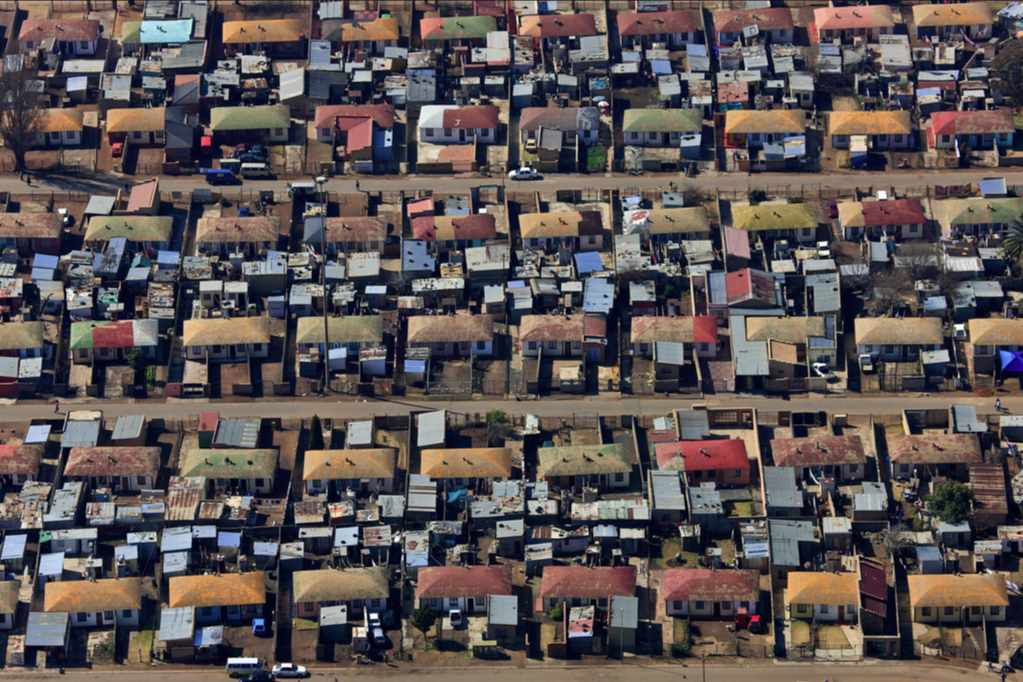
\includegraphics[scale=.25]{figures/shacks.jpg} 
%  \caption{Apartheid-Era Housing with Backyard Shacks in Soweto}
% \end{figure}

% \end{frame}

%------------------------------------------------

\begin{frame}
\frametitle{This Paper}

\centering

\begin{itemize}
  \item \textbf{Question}: What are the indirect impacts of public housing?
%  \vspace{.2cm}
%    \begin{itemize}
%      \item  Access to services, Housing growth, Nearby house prices 
%    \end{itemize}
\vspace{.3cm}

\item \textbf{Approach:} Differences-in-differences using $\sim$65 projects in Gauteng province
\vspace{3mm}
  \begin{itemize}
          \item Close/far from projects (granular spatial data)
          \item Constructed/unconstructed projects (planned/delayed/cancelled)
    \end{itemize}
% \vspace{.2cm}
% \textbf{Data and Setting:} \\
% \vspace{.1cm} 
% {\small $\sim$ 65 constructed housing projects in Gauteng province combined with GPS property transactions, building-based land information, and census data.}
\vspace{.3cm}

\item \textbf{Findings:}
  \begin{itemize}
    \item Positive direct impacts (access to water, sanitation, housing quality)
    \item No indirect impacts (nearby services, housing quality, house prices)
  \end{itemize}

\end{itemize}

\end{frame}



%\section{Background}

%------------------------------------------------

\begin{frame}
\frametitle{Public Housing in South Africa}
  \begin{itemize}
    \item 3 million houses delivered since 1994
        \begin{itemize}
          \item free-standing, single-story, two-bedrooms dwellings
          \item Undeveloped private or government-owned land
          \item $\sim$200 houses per project
        \end{itemize}
    \vspace{1mm}
    \item Eligibility: citizen, married or with dependents, monthly income $<$ R3,500, on waiting list
      \begin{itemize}
        \item Weakly enforced in practice
      \end{itemize}
    \vspace{1mm}
    \item No Resale within 7 years
      \begin{itemize}
        \item Also weakly enforced
      \end{itemize}
    \vspace{1mm}
    \item Projects are often canceled/delayed
      \begin{itemize}
        \item Miscommunication between agencies, disputes with subcontractors, failed environmental impact assessments, etc.
      \end{itemize}
  \end{itemize}
\end{frame}


% %------------------------------------------------
% \begin{frame}
% \frametitle{Who gets a house?}
%   \begin{itemize}
%     \item<1-> {\bf Official Policy:}
%     \vspace{2mm} 
%       \begin{itemize}
%         \item Must be eligible: South African Citizen, Married or with dependents, Monthly income $<$ R3,500.
%         \vspace{1mm}
%         \item National/provincial waiting lists.
%         \vspace{1mm}
%         \item No resale within 7 years.
%       \end{itemize}
%     \vspace{2mm}
%     \item<2-> {\bf In Practice}:
%       \begin{itemize}
%         \vspace{2mm} 
%         \item Wait-lists and eligibility weakly enforced, with many noted cases of corruption.
%         \vspace{1mm}
%         \item Developers often fail to meet quality requirements.
%         \vspace{1mm}
%         \item 20\% of houses not occupied by initial owners after 5 years.
%         \vspace{1mm}
%         \item More than a third have backyard shacks after 2 or less years.
%       \end{itemize}
%   \end{itemize}

% \end{frame}

% %------------------------------------------------

% \begin{frame}
% \frametitle{Canceled/Delayed Projects}
% \begin{center}

%   {\footnotesize
% {\it ``R95m down the tubes as housing project picked apart brick by brick''} \\ \hspace{20em}-- Timeslive, 2017 \\[.7em]
% {\it ``MEC Mashatile delays Munsieville Ext 5 multimillion housing project''} \\ \hspace{20em}-- DA-GPL, 2017 \\[.7em]
% {\it ``Objections put R242m housing project on hold''}\\ \hspace{20em}-- IOL News, 2016 \\[.3em]
% }
% \end{center}
% Why?
% \begin{itemize}
% \item Disputes over beneficiaries; disagreement with security contractor.
% \item Lack of  approval/coordination from all agencies.
% \item Failed environmental impact assessments.
% \end{itemize}
% \end{frame}

% %------------------------------------------------
% \section{Data and Set-up}
% %------------------------------------------------


\begin{frame}
\frametitle{Data Sources}

\begin{itemize}
  \item Gauteng Province (includes Johannesburg and Pretoria)
  \vspace{2mm}
  \begin{enumerate}
    \item Administrative map of project boundaries (2008)
    \vspace{2mm}
    \item Property Deeds Records (GPS: 2000 - 2012)
    \vspace{2mm}
    \item Census of Population (Block-level: 2001 and 2011)
    \vspace{2mm}
    \item Informal/Formal Housing (GPS: 2001 and 2011)
     \end{enumerate}

\vspace{2mm}
  \item 65 Constructed projects: contain deeds from govt sellers
    \begin{itemize}
      \item Assign construction date as modal transaction date 
    \end{itemize}
\vspace{1mm}
  \item 68 Unconstructed projects: zero deeds from govt sellers
    \begin{itemize}
      \item Assign predicted construction date from budget records
    \end{itemize}
\end{itemize}

\end{frame}

% \begin{frame}
% \frametitle{Building Census}

% \begin{figure}
%  \includegraphics[scale=.33]{figures/bblu_example.pdf} 
% \end{figure}
% \end{frame}

%------------------------------------------------

\begin{frame}
\frametitle{Housing Project Map}
\begin{center}
\begin{figure}
\frame{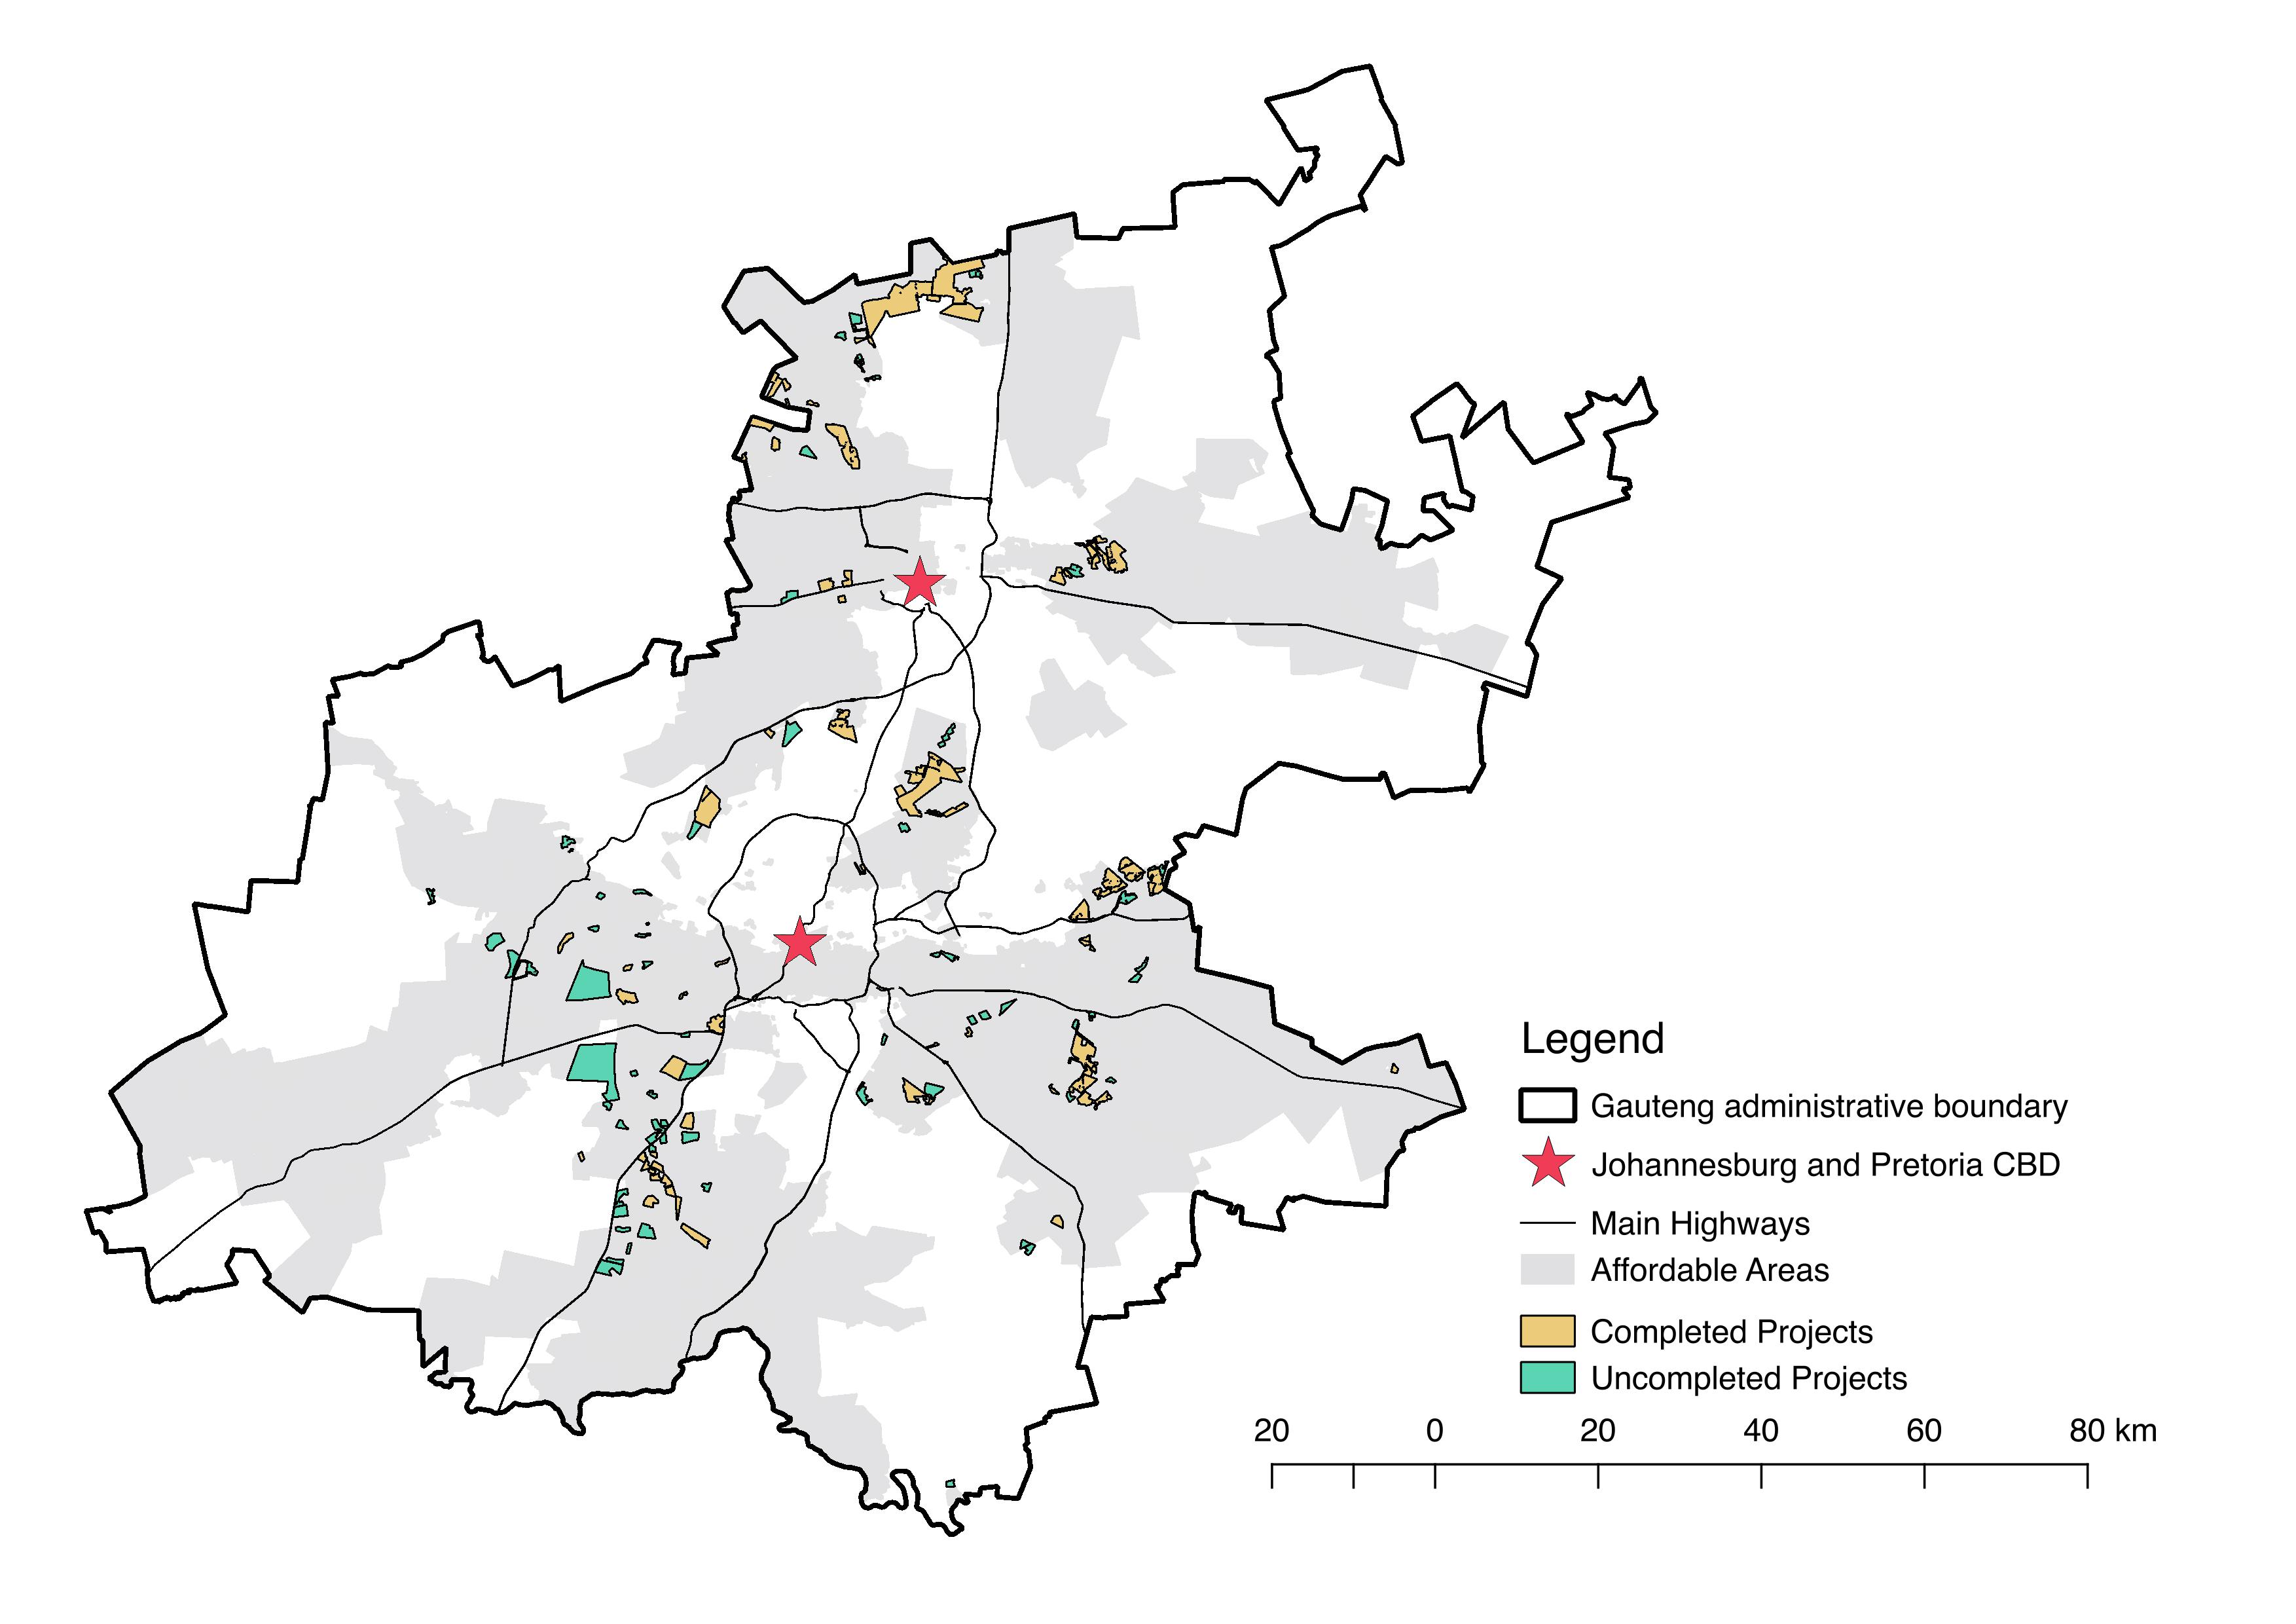
\includegraphics[scale=0.32]{datainfo/explanmap.jpg}}
\vspace{-3mm}
\end{figure}
\end{center}
\end{frame}




\begin{frame}
\frametitle{Formal Housing Density in 2001}
\centering
Formal Housing Density in 2001 \\
\vspace{.4cm} 
 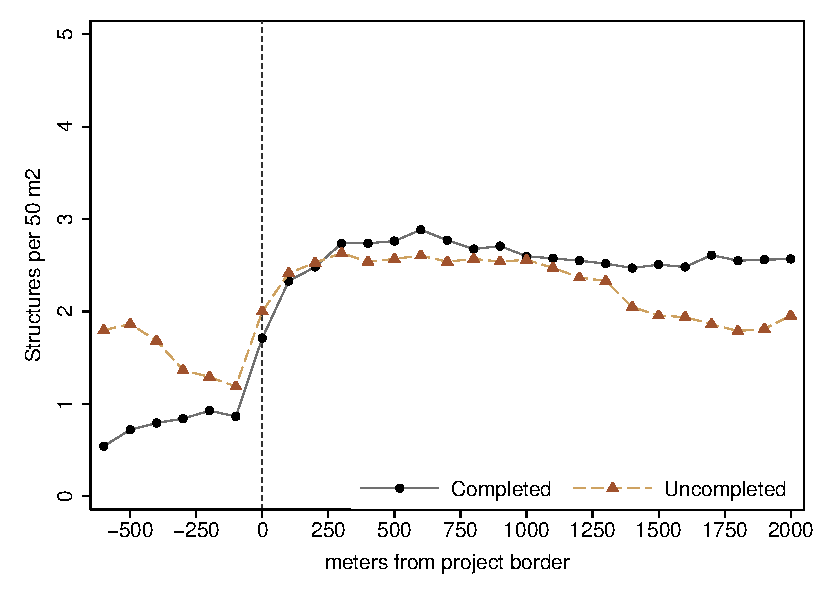
\includegraphics[width=.8\textwidth,trim={.4cm .4cm .4cm .4cm}]{figures/bblu/bblu_for_pre_means}\hspace{.5cm}

\end{frame}


\begin{frame}
\frametitle{Formal Housing Density in 2001}
\centering
Informal Housing Density in 2001 \\
\vspace{.4cm} 
 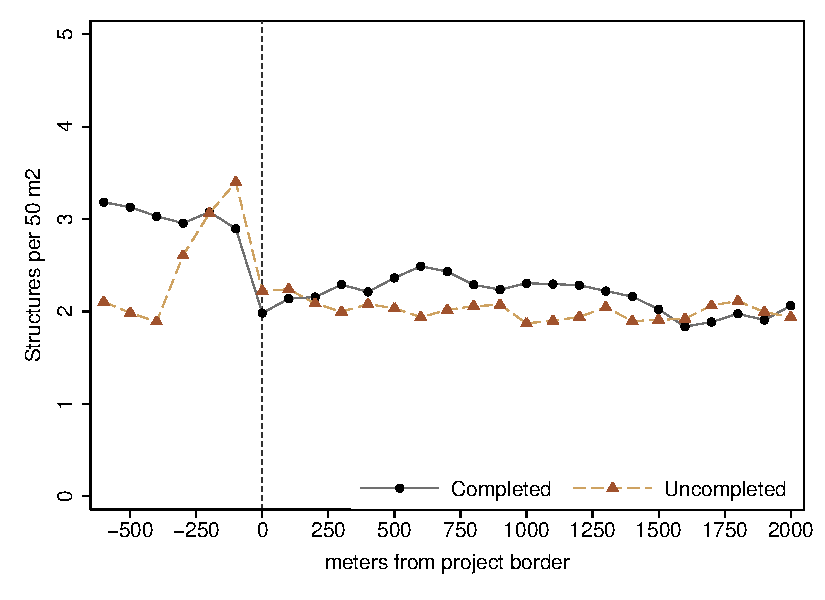
\includegraphics[width=.71\textwidth,trim={.4cm .4cm .4cm .4cm}]{figures/bblu/bblu_inf_pre_means}\hspace{.5cm}
\begin{itemize}
  \item Unconstructed projects $\rightarrow$ lower access to services at baseline (census data)
\end{itemize}

\end{frame}




% \begin{frame}
% \frametitle{Housing Density at Baseline}
% \centering
% Formal Housing Density \hspace{2cm} Informal Housing Density \\
% \vspace{.5cm}
%  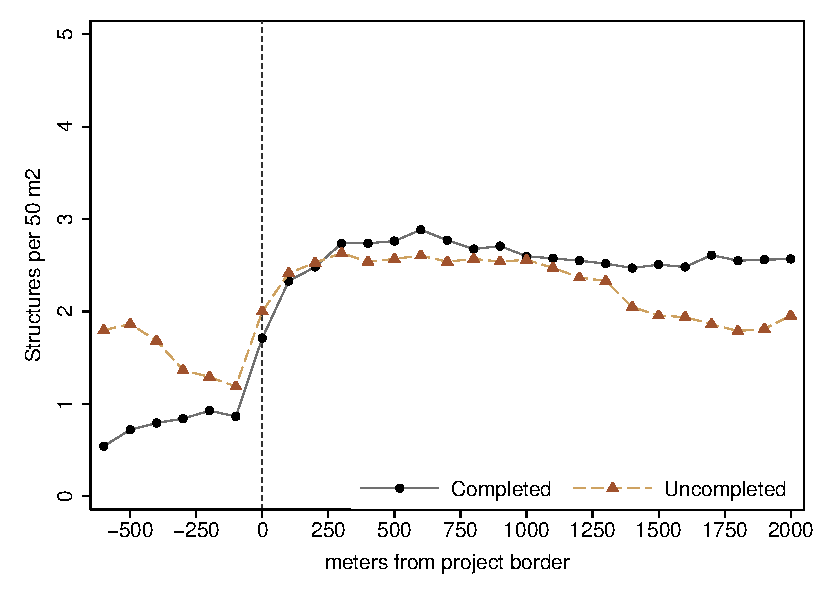
\includegraphics[width=.45\textwidth,trim={.4cm .4cm .4cm .4cm}]{figures/bblu/bblu_for_pre_means}\hspace{.5cm}
%  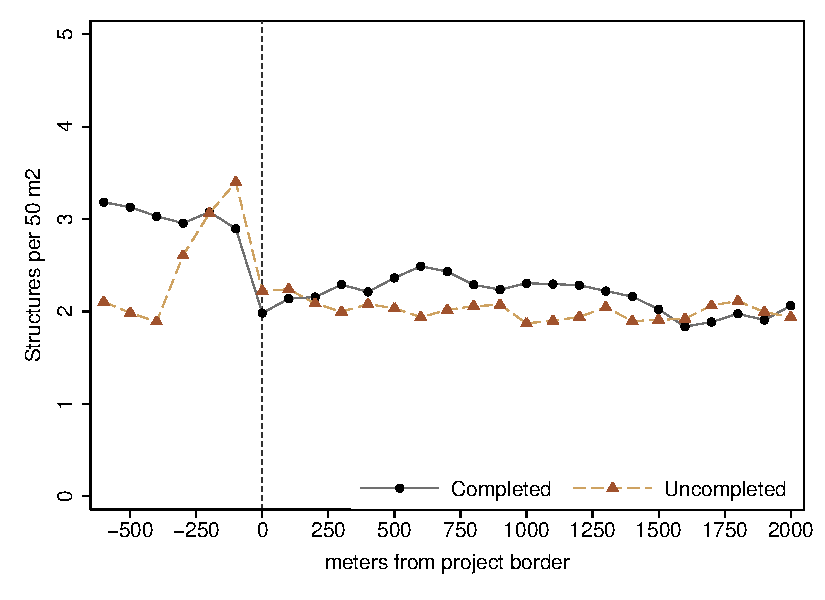
\includegraphics[width=.45\textwidth,trim={.4cm .4cm .4cm .4cm}]{figures/bblu/bblu_inf_pre_means}\hfill
% \vspace{1cm}
% \begin{itemize}
%   \item Unconstructed projects $\rightarrow$ lower access to services at baseline (census data)
% \end{itemize}
% \end{frame}

% { \footnotesize
% \begin{center}
% \vspace{2mm}
% \begin{figure}
% \centering
% Formal
% 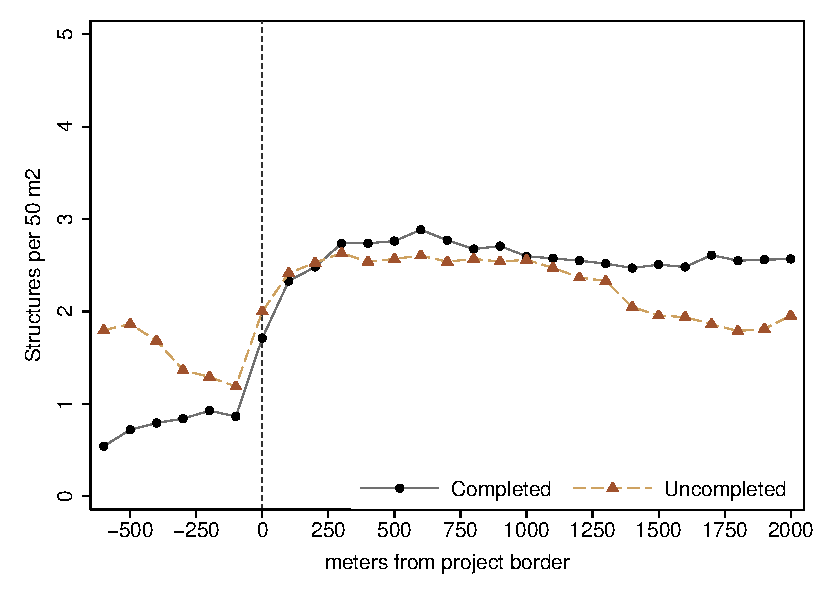
\includegraphics[width=.45\textwidth,trim={1cm 1cm 1cm 1cm}]{figures/bblu/bblu_for_pre_means}\hfill
% 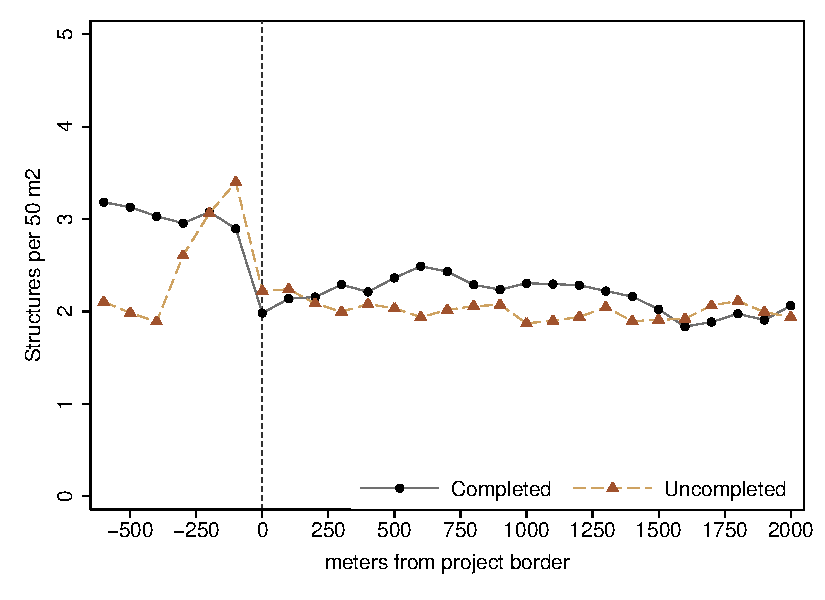
\includegraphics[width=.45\textwidth,trim={1cm 1cm 1cm 1cm}]{figures/bblu/bblu_inf_pre_means}\hfill
% %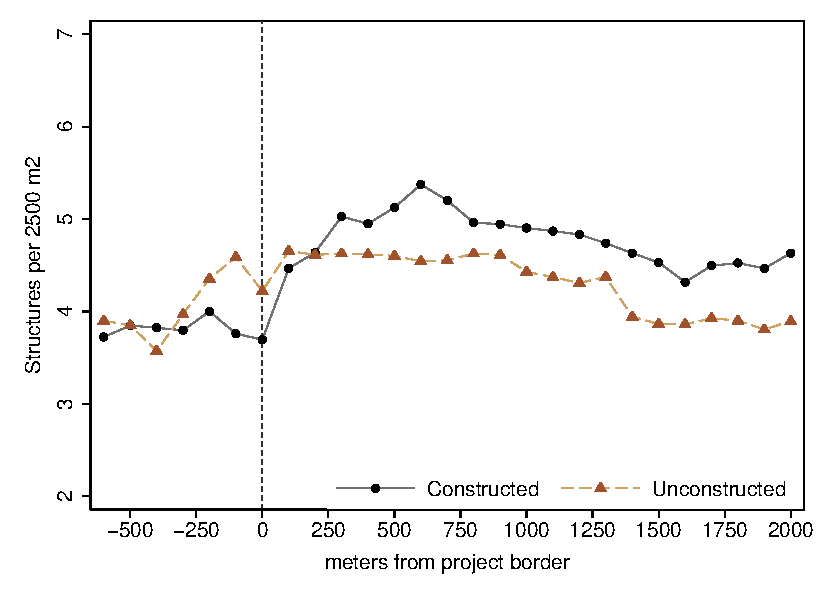
\includegraphics[width=.29\textwidth,trim={1cm 1cm 1cm 1cm}]{figures/bblu/bblu_total_buildings_pre_means}
% \caption{\scriptsize density of formal (left), informal (right) housing}
% \end{figure}
% \end{center}
% }




\begin{frame}
\frametitle{Housing Density}

\begin{equation*}
y_{ipt} \, = \, \lambda_i \, + \, \sum\limits_{d} I^d_{ipt}\Big( \alpha^d D_tC_p \, + \, \beta^dD_t\Big) \, + \, \varepsilon_{ipt}
\end{equation*}
\\with:
\begin{itemize}
\item $y_{itdp}$: housing density for cell $i$ in vicinity of project $p$ observed in year $t$.
\item $I^d_{ip}$\,=1 if cell $i$ is at distance $d$ of project $p$'s border.
\item $D_{t}\,\,$=1 if year $t$ is 2011 (post period). 
\item $C_{p}\,\,$=1 if project $p$ has been constructed.
\item $\lambda_i$: cell fixed-effect.
\item $\varepsilon_{itp}$: error term
\end{itemize}

\end{frame}

%------------------------------------------------

\begin{frame}

\only<3>{
\frametitle{Total Housing Density}
 \begin{center}
 \begin{figure}[ht]
   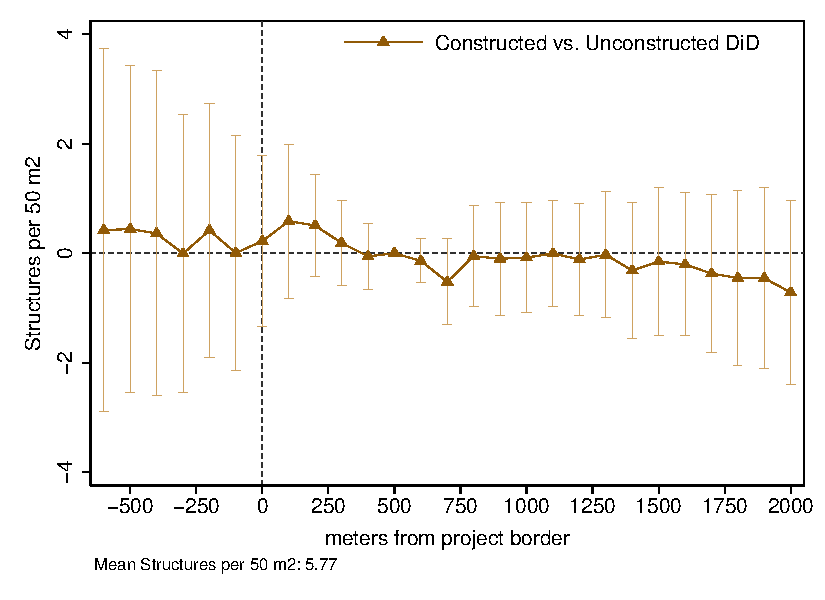
\includegraphics[scale=0.65,trim={5cm 1cm 5cm 0cm}]{figures/bblu/distplotDDD_bblu_total_buildings_admin}
   \caption{total structures}
 \end{figure}
 \end{center}
}
\only<1>{
\frametitle{Formal Housing Density}
 \begin{center}
 \begin{figure}[ht]
   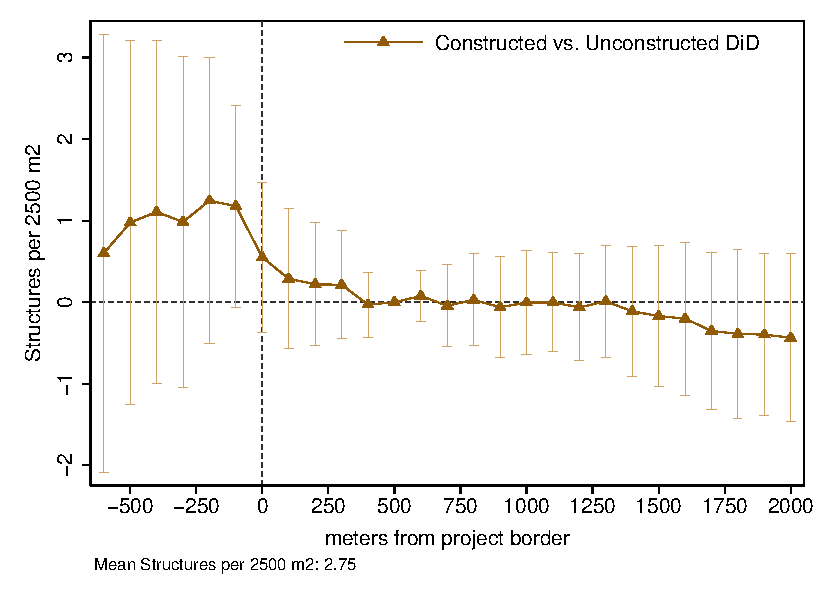
\includegraphics[scale=0.65,trim={5cm 1cm 5cm 0cm}]{figures/bblu/distplotDDD_bblu_for_admin}
   \caption{formal structures}
 \end{figure}
 \end{center}
}
\only<2>{
\frametitle{Informal Housing Density}
 \begin{center}
 \begin{figure}[ht]
   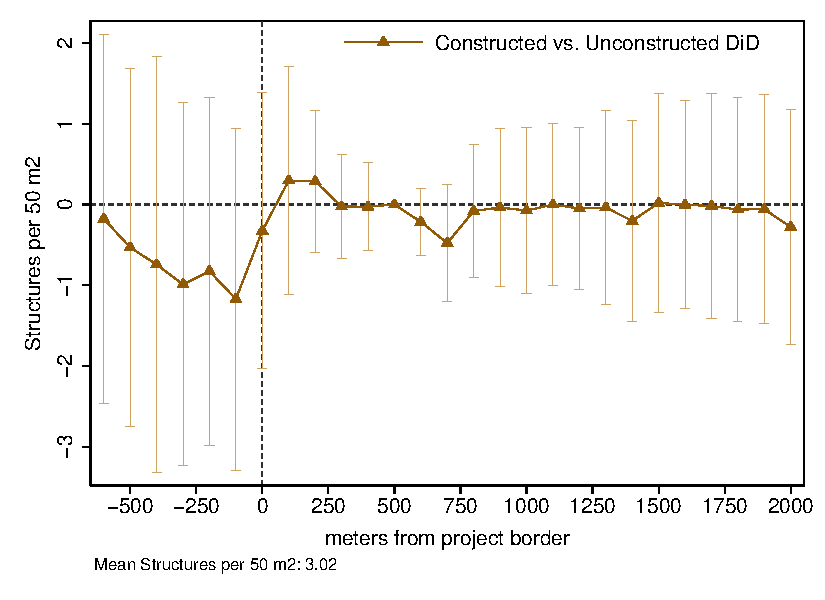
\includegraphics[scale=0.65,trim={5cm 1cm 5cm 0cm}]{figures/bblu/distplotDDD_bblu_inf_admin}
   \caption{informal structures}
 \end{figure}
 \end{center}
}
% \only<4>{
%  \begin{center}
%  \begin{figure}[ht]
%    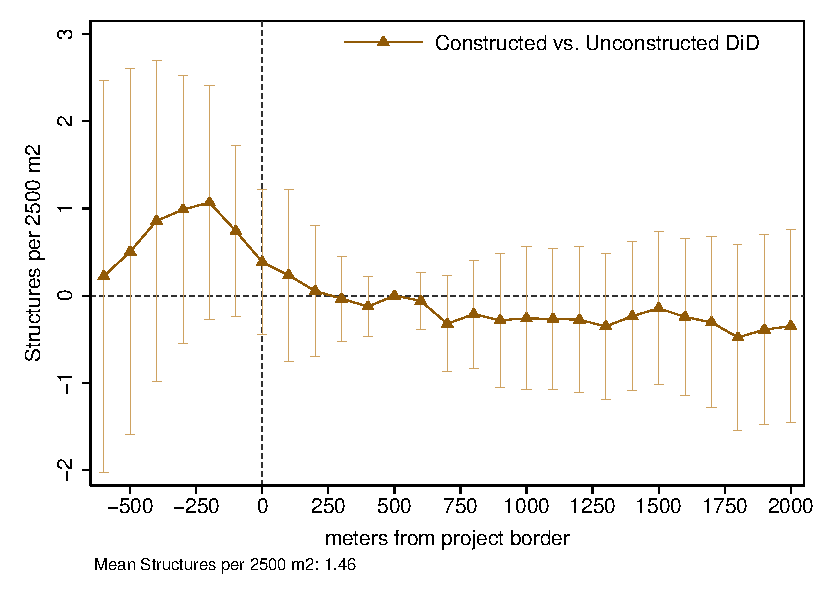
\includegraphics[scale=0.65,trim={5cm 1cm 5cm 0cm}]{figures/bblu/distplotDDD_bblu_inf_backyard_admin}
%    \caption{informal backyard structures}
%  \end{figure}
%  \end{center}
% }
% \only<5>{
%  \begin{center}
%  \begin{figure}[ht]
%    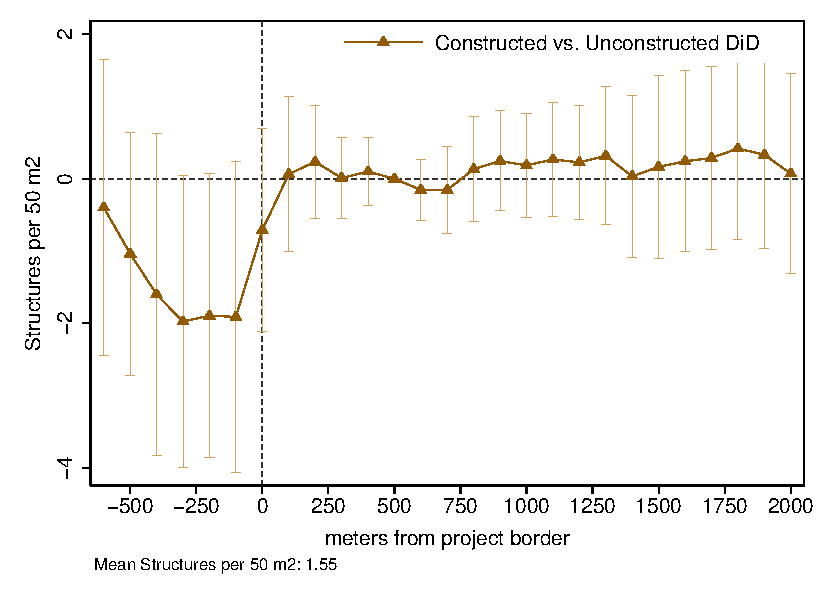
\includegraphics[scale=0.65,trim={5cm 1cm 5cm 0cm}]{figures/bblu/distplotDDD_bblu_inf_non_backyard_admin}
%    \caption{informal non-backyard structures}
%  \end{figure}
%  \end{center}
% }

\end{frame}

%------------------------------------------------

\begin{frame}
\frametitle{Triple Differences Tests}
\vspace{-1.5mm}
\begin{table}
-400m to 0m &      121.01   &      504.38** &     -383.37   &      419.94** &     -803.31***\\
            &    (296.06)   &    (206.69)   &    (292.55)   &    (181.72)   &    (265.47)   \\[0.5em]
0m to 400m  &      123.01   &       53.77   &       69.24   &       54.40   &       14.83   \\
            &    (148.32)   &    (104.60)   &    (148.03)   &    (130.97)   &    (114.79)   \\ \midrule
Mean dep. var.&    2,372.89   &    1,102.77   &    1,270.11   &      597.04   &      673.07   \\
\# Projects &         111   &         111   &         111   &         111   &         111   \\
R$^2$       &       0.098   &       0.116   &       0.055   &       0.101   &       0.044   \\
N           &     244,312   &     244,312   &     244,312   &     244,312   &     244,312   \\

\end{table}
\end{frame}





% %------------------------------------------------

\begin{frame}
\frametitle{Dwelling Characteristics (with Census Data)}
\only<1->{
\begin{equation*}
y_{hpt} \, = \, \lambda_p + \sum\limits_{e} I^e_{hpt}\Big( \alpha^e D_tC_p \, + \, \beta^eD_t \, + \, \gamma^eC_p \Big) \, + \, \varepsilon_{hpt}
\end{equation*}
}
%\, + \, \theta^e 
\only<1>{
with:
\begin{itemize}
\item $e$: {\bf project} ($>$30\% area overlap), {\bf spillover} ($\leq$30\% area overlap but within 1.5 km)
\item $y_{htp}$: Outcome for household $h$ living in vicinity of project $p$, observed in census year $t\in\{2001,2011\}$.
\item $I^e_{hpt}$=1 if household $h$ is in exposure area $e$ of project $p$.
\item $D_{t}\,\,$=1 if year $t$ is census year 2011 (post period). 
\item $C_{p}\,\,$=1 if project $p$ has been constructed.
\item $\lambda_p$: project fixed-effect.
\item $\varepsilon_{itp}$: error term.
\end{itemize}
}

\end{frame}


%------------------------------------------------

\begin{frame}
\only<1>{
\frametitle{Effect On Dwelling Characteristics }
\vspace{-1.5mm}
\begin{table}
{\footnotesize
{
\def\sym#1{\ifmmode^{#1}\else\(^{#1}\)\fi}
\begin{tabular}{l*{5}{c}}
%\hline\hline
                &\multicolumn{1}{c}{Flush}&\multicolumn{1}{c}{Water}&\multicolumn{1}{c}{Water}&\multicolumn{1}{c}{Own}&\multicolumn{1}{c}{Single}\\
                &\multicolumn{1}{c}{Toilet}&\multicolumn{1}{c}{Inside}&\multicolumn{1}{c}{Utility}&\multicolumn{1}{c}{House}&\multicolumn{1}{c}{House}\\
\hline
Proj Post Con &    0.121\sym{*}  &    0.136\sym{***}&    0.035         &   -0.085         &    0.142\sym{***}\\
                &  (0.063)         &  (0.050)         &  (0.039)         &  (0.074)         &  (0.053)         \\
[1em]
Spill Post Con &    0.037         &    0.031         &   -0.012         &   -0.008         &    0.015         \\
                &  (0.035)         &  (0.033)         &  (0.012)         &  (0.028)         &  (0.029)         \\
\hline
N               &2,020,549         &2,020,549         &2,020,549       &1,958,335         &1,936,911         \\
Mean2001        &    0.699         &    0.300         &    0.947         &    0.507         &    0.535         \\
Mean2011        &    0.807         &    0.481         &    0.941         &    0.442         &    0.622         \\
\hline
%\hline
\multicolumn{6}{l}{\footnotesize Standard errors clustered at the project-level in parentheses}\\
\multicolumn{6}{l}{\footnotesize \sym{*} \(p<0.10\), \sym{**} \(p<0.05\), \sym{***} \(p<0.01\)}\\
\end{tabular}
}

}
\end{table}
}
\only<2>{
\frametitle{Effect On Dwelling Characteristics }
\vspace{-1.5mm}
\begin{table}
{\footnotesize
{
\def\sym#1{\ifmmode^{#1}\else\(^{#1}\)\fi}
\begin{tabular}{l*{3}{c}}
%\hline\hline
               &\multicolumn{1}{c}{Elec.}&\multicolumn{1}{c}{HH}&\multicolumn{1}{c}{Pop}\\
		&\multicolumn{1}{c}{Cooking}&\multicolumn{1}{c}{Density}&\multicolumn{1}{c}{Density}\\
\hline
Proj Post Const &    0.290\sym{***}      &   24.9         &   43.5        \\
 &  (0.069)             &(784)         &(1,466)         \\
[1em]
Spill Post Const &    0.042          &  294.7        &  442.2         \\
			 &  (0.033)           &(206)         &(469)         \\
\hline
N               &2,020,549           &9,669         &9,669        \\
Mean2001        &    0.570             &2,230         &7,365    \\
Mean2011       &    0.811             &3,188      &9,162       \\
\hline
%\hline
\multicolumn{4}{l}{\footnotesize Standard errors clustered at the project-level in parentheses}\\
\multicolumn{4}{l}{\footnotesize \sym{*} \(p<0.10\), \sym{**} \(p<0.05\), \sym{***} \(p<0.01\)}\\
\end{tabular}
}

}
\end{table}
}
\end{frame}

\begin{frame}
\frametitle{Price Effects}
\begin{equation*}
\begin{split}
P_{ipt} \, = & \,\,\,  \sum\limits_{d} I^d_{ipt}\Big( \alpha^d D^1_tC^1_p \, + \, \beta^dD^1_tC^0_p + \, \gamma^dD^0_tC^1_p \, + \, \theta^dD^0_tC^0_p \Big ) \\ 
&\quad\quad\quad\quad\quad\quad\quad\quad\quad + \, \lambda_p \,  + \, \eta_{t} \, +\,  X^{'}_{i}\phi \, + \, \varepsilon_{ipt}
\end{split}
\end{equation*}

\begin{itemize}
\item $P_{itp}$: log-price of property $i$ sold at time $t$, in vicinity of project $p$.
\item $I^d_{ip}$\,=1 if property $i$ is at distance $d$ of project $p$'s border.
\item $D^j_{t}$ =1 if date $t$ is before ($j=0$) or after ($j=1$) construction. 
\item $C^j_{p}\,\,$ =1 if project $p$ unconstructed ($j=1$) of constructed ($j=0$).
\item $X_{i}$: quadratic in lot size of property $i$.
\item $\lambda_p$: project fixed-effect.
\item $\eta_{t}$: time (year$\,\times\,$month) fixed-effect.

\item $\varepsilon_{itp}$: error term
\end{itemize}
\end{frame}

%------------------------------------------------

\begin{frame}

\only<1>{
\frametitle{Price and Distance: Constructed Projects}
\centering
Constructed Projects \\
\vspace{.2cm}
% \begin{center}
% \begin{figure}[ht]
   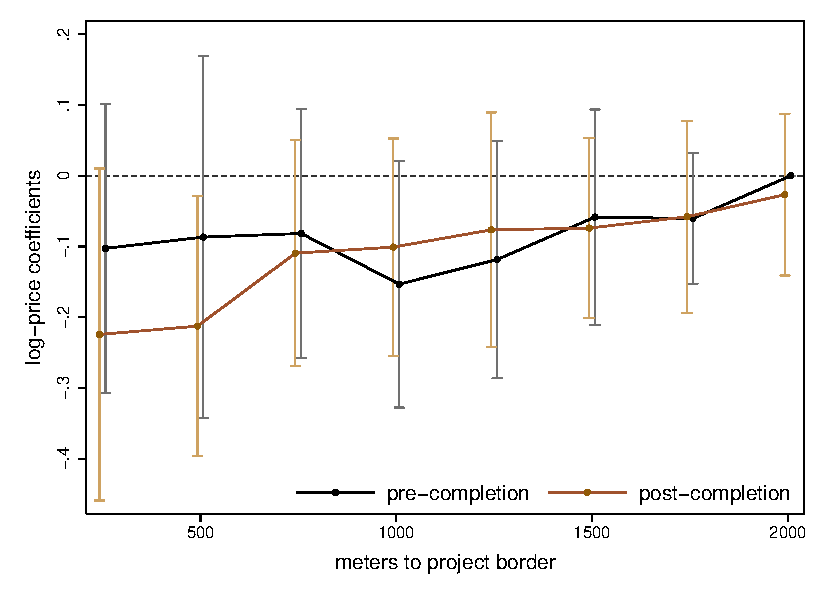
\includegraphics[scale=0.65,trim={5cm 1cm 5cm 0cm}]{figures/gradplot/distance_plot_rdp}
%   \caption{proximity effects: constructed projects}
% \end{figure}
% \end{center}
}
\only<2>{
\frametitle{Price and Distance: Unconstructed Projects}
\centering
Unconstructed Projects \\
\vspace{.2cm}
% \begin{center}
% \begin{figure}[ht]
   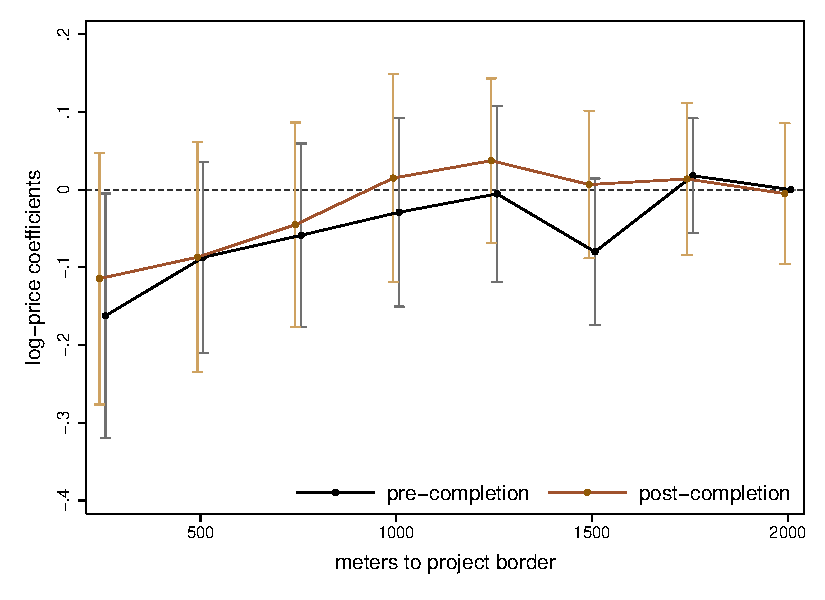
\includegraphics[scale=0.65,trim={5cm 1cm 5cm 0cm}]{figures/gradplot/distance_plot_placebo}
%   \caption{proximity effects: non-constructed projects}
% \end{figure}
% \end{center}
}
\only<3>{
\frametitle{Price and Time: Constructed Projects}
\centering
Constructed Projects \\
\vspace{.2cm}
% \begin{center}
% \begin{figure}[ht]
   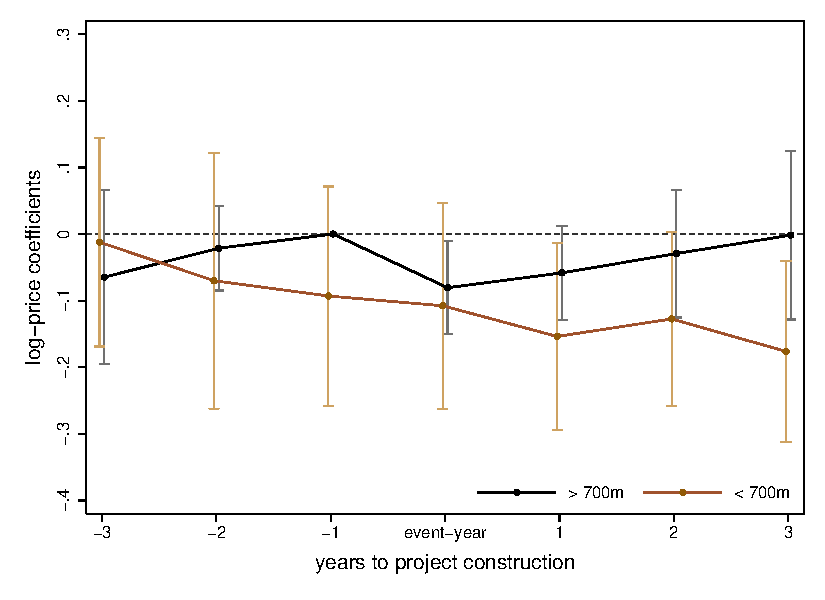
\includegraphics[scale=0.65,trim={5cm 1cm 5cm 0cm}]{figures/gradplot/time_plot_rdp}
%   \caption{timing effects: constructed projects}
% \end{figure}
% \end{center}
}
\only<4>{
\frametitle{Price and Time: Unconstructed Projects}
\centering
Unconstructed Projects \\
\vspace{.2cm}
% \begin{center}
% \begin{figure}[ht]
   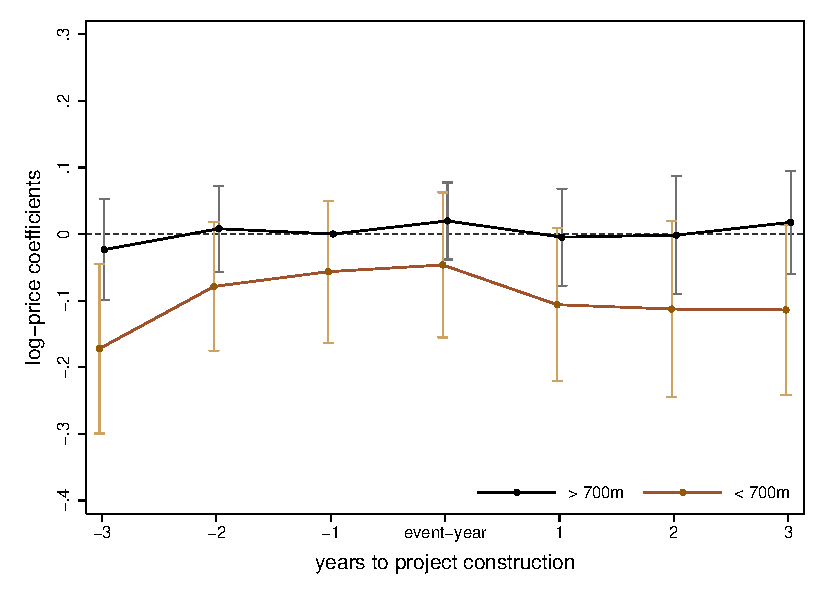
\includegraphics[scale=0.65,trim={5cm 1cm 5cm 0cm}]{figures/gradplot/time_plot_placebo}
%   \caption{timing effects: non-constructed projects}
% \end{figure}
% \end{center}
}
\end{frame}

%------------------------------------------------

\begin{frame}
\frametitle{Summary \& Conclusion}

Main Takeaway:
\begin{itemize}
\item Public housing effective tool to crowd-out slum development, but limited spillover benefits.
 \end{itemize}
\vspace{2mm}
Next Steps:
  \begin{itemize}
    \item Cost/Benefit calculations 
    \item Heterogeneity 
    \item Mechanisms
  \end{itemize}

{\Large
  \begin{center}
  Thank You!
  \end{center}
}
\end{frame}

%------------------------------------------------

\end{document} 
